\documentclass[1p]{elsarticle_modified}
%\bibliographystyle{elsarticle-num}

%\usepackage[colorlinks]{hyperref}
%\usepackage{abbrmath_seonhwa} %\Abb, \Ascr, \Acal ,\Abf, \Afrak
\usepackage{amsfonts}
\usepackage{amssymb}
\usepackage{amsmath}
\usepackage{amsthm}
\usepackage{scalefnt}
\usepackage{amsbsy}
\usepackage{kotex}
\usepackage{caption}
\usepackage{subfig}
\usepackage{color}
\usepackage{graphicx}
\usepackage{xcolor} %% white, black, red, green, blue, cyan, magenta, yellow
\usepackage{float}
\usepackage{setspace}
\usepackage{hyperref}

\usepackage{tikz}
\usetikzlibrary{arrows}

\usepackage{multirow}
\usepackage{array} % fixed length table
\usepackage{hhline}

%%%%%%%%%%%%%%%%%%%%%
\makeatletter
\renewcommand*\env@matrix[1][\arraystretch]{%
	\edef\arraystretch{#1}%
	\hskip -\arraycolsep
	\let\@ifnextchar\new@ifnextchar
	\array{*\c@MaxMatrixCols c}}
\makeatother %https://tex.stackexchange.com/questions/14071/how-can-i-increase-the-line-spacing-in-a-matrix
%%%%%%%%%%%%%%%

\usepackage[normalem]{ulem}

\newcommand{\msout}[1]{\ifmmode\text{\sout{\ensuremath{#1}}}\else\sout{#1}\fi}
%SOURCE: \msout is \stkout macro in https://tex.stackexchange.com/questions/20609/strikeout-in-math-mode

\newcommand{\cancel}[1]{
	\ifmmode
	{\color{red}\msout{#1}}
	\else
	{\color{red}\sout{#1}}
	\fi
}

\newcommand{\add}[1]{
	{\color{blue}\uwave{#1}}
}

\newcommand{\replace}[2]{
	\ifmmode
	{\color{red}\msout{#1}}{\color{blue}\uwave{#2}}
	\else
	{\color{red}\sout{#1}}{\color{blue}\uwave{#2}}
	\fi
}

\newcommand{\Sol}{\mathcal{S}} %segment
\newcommand{\D}{D} %diagram
\newcommand{\A}{\mathcal{A}} %arc


%%%%%%%%%%%%%%%%%%%%%%%%%%%%%5 test

\def\sl{\operatorname{\textup{SL}}(2,\Cbb)}
\def\psl{\operatorname{\textup{PSL}}(2,\Cbb)}
\def\quan{\mkern 1mu \triangleright \mkern 1mu}

\theoremstyle{definition}
\newtheorem{thm}{Theorem}[section]
\newtheorem{prop}[thm]{Proposition}
\newtheorem{lem}[thm]{Lemma}
\newtheorem{ques}[thm]{Question}
\newtheorem{cor}[thm]{Corollary}
\newtheorem{defn}[thm]{Definition}
\newtheorem{exam}[thm]{Example}
\newtheorem{rmk}[thm]{Remark}
\newtheorem{alg}[thm]{Algorithm}

\newcommand{\I}{\sqrt{-1}}
\begin{document}

%\begin{frontmatter}
%
%\title{Boundary parabolic representations of knots up to 8 crossings}
%
%%% Group authors per affiliation:
%\author{Yunhi Cho} 
%\address{Department of Mathematics, University of Seoul, Seoul, Korea}
%\ead{yhcho@uos.ac.kr}
%
%
%\author{Seonhwa Kim} %\fnref{s_kim}}
%\address{Center for Geometry and Physics, Institute for Basic Science, Pohang, 37673, Korea}
%\ead{ryeona17@ibs.re.kr}
%
%\author{Hyuk Kim}
%\address{Department of Mathematical Sciences, Seoul National University, Seoul 08826, Korea}
%\ead{hyukkim@snu.ac.kr}
%
%\author{Seokbeom Yoon}
%\address{Department of Mathematical Sciences, Seoul National University, Seoul, 08826,  Korea}
%\ead{sbyoon15@snu.ac.kr}
%
%\begin{abstract}
%We find all boundary parabolic representation of knots up to 8 crossings.
%
%\end{abstract}
%\begin{keyword}
%    \MSC[2010] 57M25 
%\end{keyword}
%
%\end{frontmatter}

%\linenumbers
%\tableofcontents
%
\newcommand\colored[1]{\textcolor{white}{\rule[-0.35ex]{0.8em}{1.4ex}}\kern-0.8em\color{red} #1}%
%\newcommand\colored[1]{\textcolor{white}{ #1}\kern-2.17ex	\textcolor{white}{ #1}\kern-1.81ex	\textcolor{white}{ #1}\kern-2.15ex\color{red}#1	}

{\Large $\underline{11n_{52}~(K11n_{52})}$}

\setlength{\tabcolsep}{10pt}
\renewcommand{\arraystretch}{1.6}
\vspace{1cm}\begin{tabular}{m{100pt}>{\centering\arraybackslash}m{274pt}}
\multirow{5}{120pt}{
	\centering
	\includegraphics[width=112pt]{../../../GIT/diagram.site/Diagrams/png/668_11n_52.png}\\
\ \ \ A knot diagram\footnotemark}&
\allowdisplaybreaks
\textbf{Linearized knot diagam} \\
\cline{2-2}
 &
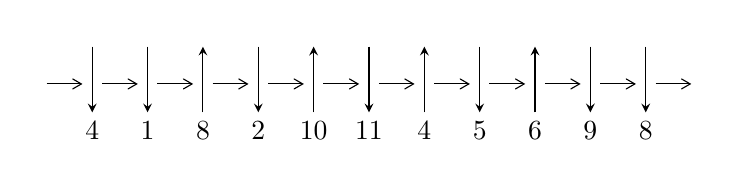
\begin{tikzpicture}[x=20pt, y=17pt]
	% nodes
	\node (C0) at (0, 0) {};
	\node (C1) at (1, 0) {};
	\node (C1U) at (1, +1) {};
	\node (C1D) at (1, -1) {4};

	\node (C2) at (2, 0) {};
	\node (C2U) at (2, +1) {};
	\node (C2D) at (2, -1) {1};

	\node (C3) at (3, 0) {};
	\node (C3U) at (3, +1) {};
	\node (C3D) at (3, -1) {8};

	\node (C4) at (4, 0) {};
	\node (C4U) at (4, +1) {};
	\node (C4D) at (4, -1) {2};

	\node (C5) at (5, 0) {};
	\node (C5U) at (5, +1) {};
	\node (C5D) at (5, -1) {10};

	\node (C6) at (6, 0) {};
	\node (C6U) at (6, +1) {};
	\node (C6D) at (6, -1) {11};

	\node (C7) at (7, 0) {};
	\node (C7U) at (7, +1) {};
	\node (C7D) at (7, -1) {4};

	\node (C8) at (8, 0) {};
	\node (C8U) at (8, +1) {};
	\node (C8D) at (8, -1) {5};

	\node (C9) at (9, 0) {};
	\node (C9U) at (9, +1) {};
	\node (C9D) at (9, -1) {6};

	\node (C10) at (10, 0) {};
	\node (C10U) at (10, +1) {};
	\node (C10D) at (10, -1) {9};

	\node (C11) at (11, 0) {};
	\node (C11U) at (11, +1) {};
	\node (C11D) at (11, -1) {8};
	\node (C12) at (12, 0) {};

	% arrows
	\draw[->,>={angle 60}]
	(C0) edge (C1) (C1) edge (C2) (C2) edge (C3) (C3) edge (C4) (C4) edge (C5) (C5) edge (C6) (C6) edge (C7) (C7) edge (C8) (C8) edge (C9) (C9) edge (C10) (C10) edge (C11) (C11) edge (C12) ;	\draw[->,>=stealth]
	(C1U) edge (C1D) (C2U) edge (C2D) (C3D) edge (C3U) (C4U) edge (C4D) (C5D) edge (C5U) (C6U) edge (C6D) (C7D) edge (C7U) (C8U) edge (C8D) (C9D) edge (C9U) (C10U) edge (C10D) (C11U) edge (C11D) ;
	\end{tikzpicture} \\
\hhline{~~} \\& 
\textbf{Solving Sequence} \\ \cline{2-2} 
 &
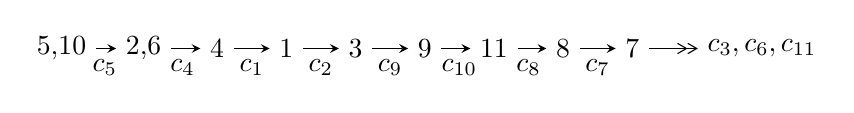
\begin{tikzpicture}[x=25pt, y=7pt]
	% node
	\node (A0) at (-1/8, 0) {5,10};
	\node (A1) at (17/16, 0) {2,6};
	\node (A2) at (17/8, 0) {4};
	\node (A3) at (25/8, 0) {1};
	\node (A4) at (33/8, 0) {3};
	\node (A5) at (41/8, 0) {9};
	\node (A6) at (49/8, 0) {11};
	\node (A7) at (57/8, 0) {8};
	\node (A8) at (65/8, 0) {7};
	\node (C1) at (1/2, -1) {$c_{5}$};
	\node (C2) at (13/8, -1) {$c_{4}$};
	\node (C3) at (21/8, -1) {$c_{1}$};
	\node (C4) at (29/8, -1) {$c_{2}$};
	\node (C5) at (37/8, -1) {$c_{9}$};
	\node (C6) at (45/8, -1) {$c_{10}$};
	\node (C7) at (53/8, -1) {$c_{8}$};
	\node (C8) at (61/8, -1) {$c_{7}$};
	\node (A9) at (10, 0) {$c_{3},c_{6},c_{11}$};

	% edge
	\draw[->,>=stealth]	
	(A0) edge (A1) (A1) edge (A2) (A2) edge (A3) (A3) edge (A4) (A4) edge (A5) (A5) edge (A6) (A6) edge (A7) (A7) edge (A8) ;
	\draw[->>,>={angle 60}]	
	(A8) edge (A9);
\end{tikzpicture} \\ 

\end{tabular} \\

\footnotetext{
The image of knot diagram is generated by the software ``\textbf{Draw programme}" developed by Andrew Bartholomew(\url{http://www.layer8.co.uk/maths/draw/index.htm\#Running-draw}), where we modified some parts for our purpose(\url{https://github.com/CATsTAILs/LinksPainter}).
}\phantom \\ \newline 
\centering \textbf{Ideals for irreducible components\footnotemark of $X_{\text{par}}$} 
 
\begin{align*}
I^u_{1}&=\langle 
- u^{32}- u^{31}+\cdots+b+u,\;- u^{32}- u^{31}+\cdots+a-1,\;u^{34}+2 u^{33}+\cdots-2 u-1\rangle \\
I^u_{2}&=\langle 
b+1,\;- u^3+u^2+a- u+2,\;u^5- u^4+2 u^3- u^2+u-1\rangle \\
\\
\end{align*}
\raggedright * 2 irreducible components of $\dim_{\mathbb{C}}=0$, with total 39 representations.\\
\footnotetext{All coefficients of polynomials are rational numbers. But the coefficients are sometimes approximated in decimal forms when there is not enough margin.}
\newpage
\renewcommand{\arraystretch}{1}
\centering \section*{I. $I^u_{1}= \langle - u^{32}- u^{31}+\cdots+b+u,\;- u^{32}- u^{31}+\cdots+a-1,\;u^{34}+2 u^{33}+\cdots-2 u-1 \rangle$}
\flushleft \textbf{(i) Arc colorings}\\
\begin{tabular}{m{7pt} m{180pt} m{7pt} m{180pt} }
\flushright $a_{5}=$&$\begin{pmatrix}1\\0\end{pmatrix}$ \\
\flushright $a_{10}=$&$\begin{pmatrix}0\\u\end{pmatrix}$ \\
\flushright $a_{2}=$&$\begin{pmatrix}u^{32}+u^{31}+\cdots-5 u^3+1\\u^{32}+u^{31}+\cdots- u^2- u\end{pmatrix}$ \\
\flushright $a_{6}=$&$\begin{pmatrix}1\\- u^2\end{pmatrix}$ \\
\flushright $a_{4}=$&$\begin{pmatrix}-2 u^{32}-2 u^{31}+\cdots+u^2+u\\- u^{32}- u^{31}+\cdots+u^2+2 u\end{pmatrix}$ \\
\flushright $a_{1}=$&$\begin{pmatrix}- u^{11}-2 u^9-2 u^7- u^3\\- u^{11}-3 u^9-4 u^7- u^5+u^3+u\end{pmatrix}$ \\
\flushright $a_{3}=$&$\begin{pmatrix}4 u^{32}+4 u^{31}+\cdots-3 u-1\\2 u^{32}+u^{31}+\cdots- u^2-3 u\end{pmatrix}$ \\
\flushright $a_{9}=$&$\begin{pmatrix}- u\\u^3+u\end{pmatrix}$ \\
\flushright $a_{11}=$&$\begin{pmatrix}- u^3\\u^5+u^3+u\end{pmatrix}$ \\
\flushright $a_{8}=$&$\begin{pmatrix}u^3\\u^3+u\end{pmatrix}$ \\
\flushright $a_{7}=$&$\begin{pmatrix}- u^6- u^4+1\\u^8+2 u^6+2 u^4\end{pmatrix}$\\ \flushright $a_{7}=$&$\begin{pmatrix}- u^6- u^4+1\\u^8+2 u^6+2 u^4\end{pmatrix}$\\&\end{tabular}
\flushleft \textbf{(ii) Obstruction class $= -1$}\\~\\
\flushleft \textbf{(iii) Cusp Shapes $= -4 u^{33}-11 u^{32}-46 u^{31}-97 u^{30}-238 u^{29}-421 u^{28}-758 u^{27}-1154 u^{26}-1651 u^{25}-2191 u^{24}-2586 u^{23}-2978 u^{22}-2933 u^{21}-2856 u^{20}-2304 u^{19}-1728 u^{18}-973 u^{17}-263 u^{16}+258 u^{15}+646 u^{14}+764 u^{13}+710 u^{12}+560 u^{11}+314 u^{10}+160 u^9+16 u^8-52 u^7-64 u^6-51 u^5-4 u^4+16 u^3+18 u^2+15 u+3$}\\~\\
\newpage\renewcommand{\arraystretch}{1}
\flushleft \textbf{(iv) u-Polynomials at the component}\newline \\
\begin{tabular}{m{50pt}|m{274pt}}
Crossings & \hspace{64pt}u-Polynomials at each crossing \\
\hline $$\begin{aligned}c_{1},c_{4}\end{aligned}$$&$\begin{aligned}
&u^{34}-6 u^{33}+\cdots+4 u-1
\end{aligned}$\\
\hline $$\begin{aligned}c_{2}\end{aligned}$$&$\begin{aligned}
&u^{34}+10 u^{33}+\cdots+2 u^2+1
\end{aligned}$\\
\hline $$\begin{aligned}c_{3},c_{7}\end{aligned}$$&$\begin{aligned}
&u^{34}- u^{33}+\cdots+32 u+32
\end{aligned}$\\
\hline $$\begin{aligned}c_{5},c_{9}\end{aligned}$$&$\begin{aligned}
&u^{34}-2 u^{33}+\cdots+2 u-1
\end{aligned}$\\
\hline $$\begin{aligned}c_{6},c_{8}\end{aligned}$$&$\begin{aligned}
&u^{34}+2 u^{33}+\cdots-58 u-17
\end{aligned}$\\
\hline $$\begin{aligned}c_{10}\end{aligned}$$&$\begin{aligned}
&u^{34}+18 u^{33}+\cdots+2 u+1
\end{aligned}$\\
\hline $$\begin{aligned}c_{11}\end{aligned}$$&$\begin{aligned}
&u^{34}-2 u^{33}+\cdots+2 u+1
\end{aligned}$\\
\hline
\end{tabular}\\~\\
\newpage\renewcommand{\arraystretch}{1}
\flushleft \textbf{(v) Riley Polynomials at the component}\newline \\
\begin{tabular}{m{50pt}|m{274pt}}
Crossings & \hspace{64pt}Riley Polynomials at each crossing \\
\hline $$\begin{aligned}c_{1},c_{4}\end{aligned}$$&$\begin{aligned}
&y^{34}-10 y^{33}+\cdots+2 y^2+1
\end{aligned}$\\
\hline $$\begin{aligned}c_{2}\end{aligned}$$&$\begin{aligned}
&y^{34}+34 y^{33}+\cdots+4 y+1
\end{aligned}$\\
\hline $$\begin{aligned}c_{3},c_{7}\end{aligned}$$&$\begin{aligned}
&y^{34}-33 y^{33}+\cdots-11776 y+1024
\end{aligned}$\\
\hline $$\begin{aligned}c_{5},c_{9}\end{aligned}$$&$\begin{aligned}
&y^{34}+18 y^{33}+\cdots+2 y+1
\end{aligned}$\\
\hline $$\begin{aligned}c_{6},c_{8}\end{aligned}$$&$\begin{aligned}
&y^{34}-22 y^{33}+\cdots+682 y+289
\end{aligned}$\\
\hline $$\begin{aligned}c_{10}\end{aligned}$$&$\begin{aligned}
&y^{34}-2 y^{33}+\cdots-18 y+1
\end{aligned}$\\
\hline $$\begin{aligned}c_{11}\end{aligned}$$&$\begin{aligned}
&y^{34}+38 y^{33}+\cdots+2 y+1
\end{aligned}$\\
\hline
\end{tabular}\\~\\
\newpage\flushleft \textbf{(vi) Complex Volumes and Cusp Shapes}
$$\begin{array}{c|c|c}  
\text{Solutions to }I^u_{1}& \I (\text{vol} + \sqrt{-1}CS) & \text{Cusp shape}\\
 \hline 
\begin{aligned}
u &= -0.392064 + 0.911772 I \\
a &= -1.220400 + 0.149546 I \\
b &= -0.151137 - 0.378084 I\end{aligned}
 & -0.33123 - 1.99737 I & -1.04171 + 3.94659 I \\ \hline\begin{aligned}
u &= -0.392064 - 0.911772 I \\
a &= -1.220400 - 0.149546 I \\
b &= -0.151137 + 0.378084 I\end{aligned}
 & -0.33123 + 1.99737 I & -1.04171 - 3.94659 I \\ \hline\begin{aligned}
u &= \phantom{-}0.643857 + 0.740919 I \\
a &= \phantom{-}0.444510 + 0.058747 I \\
b &= -0.919309 - 0.963610 I\end{aligned}
 & \phantom{-}7.32303 - 1.01150 I & \phantom{-}0.462803 - 0.538404 I \\ \hline\begin{aligned}
u &= \phantom{-}0.643857 - 0.740919 I \\
a &= \phantom{-}0.444510 - 0.058747 I \\
b &= -0.919309 + 0.963610 I\end{aligned}
 & \phantom{-}7.32303 + 1.01150 I & \phantom{-}0.462803 + 0.538404 I \\ \hline\begin{aligned}
u &= \phantom{-}0.631061 + 0.814143 I \\
a &= -1.09866 - 1.38992 I \\
b &= -0.986984 + 0.934448 I\end{aligned}
 & \phantom{-}7.11131 + 5.93371 I & -0.19300 - 5.69756 I \\ \hline\begin{aligned}
u &= \phantom{-}0.631061 - 0.814143 I \\
a &= -1.09866 + 1.38992 I \\
b &= -0.986984 - 0.934448 I\end{aligned}
 & \phantom{-}7.11131 - 5.93371 I & -0.19300 + 5.69756 I \\ \hline\begin{aligned}
u &= -0.820098 + 0.217356 I \\
a &= -1.021230 - 0.783883 I \\
b &= -1.088070 + 0.833628 I\end{aligned}
 & \phantom{-}3.98565 + 7.54944 I & -1.73478 - 4.55602 I \\ \hline\begin{aligned}
u &= -0.820098 - 0.217356 I \\
a &= -1.021230 + 0.783883 I \\
b &= -1.088070 - 0.833628 I\end{aligned}
 & \phantom{-}3.98565 - 7.54944 I & -1.73478 + 4.55602 I \\ \hline\begin{aligned}
u &= -0.775445 + 0.276843 I \\
a &= -0.000113 + 0.147223 I \\
b &= -0.749373 - 0.980750 I\end{aligned}
 & \phantom{-}5.05465 + 0.88184 I & -0.0341976 + 0.1167760 I \\ \hline\begin{aligned}
u &= -0.775445 - 0.276843 I \\
a &= -0.000113 - 0.147223 I \\
b &= -0.749373 + 0.980750 I\end{aligned}
 & \phantom{-}5.05465 - 0.88184 I & -0.0341976 - 0.1167760 I\\
 \hline 
 \end{array}$$\newpage$$\begin{array}{c|c|c}  
\text{Solutions to }I^u_{1}& \I (\text{vol} + \sqrt{-1}CS) & \text{Cusp shape}\\
 \hline 
\begin{aligned}
u &= -0.255241 + 1.154760 I \\
a &= -1.63194 - 0.61364 I \\
b &= -0.719802 - 0.838712 I\end{aligned}
 & \phantom{-}0.59034 - 2.20193 I & -5.39762 + 2.89255 I \\ \hline\begin{aligned}
u &= -0.255241 - 1.154760 I \\
a &= -1.63194 + 0.61364 I \\
b &= -0.719802 + 0.838712 I\end{aligned}
 & \phantom{-}0.59034 + 2.20193 I & -5.39762 - 2.89255 I \\ \hline\begin{aligned}
u &= \phantom{-}0.401589 + 1.121620 I \\
a &= \phantom{-}0.740490 + 0.229483 I \\
b &= \phantom{-}0.867707 + 0.523486 I\end{aligned}
 & -4.35229 + 1.60461 I & -8.26502 - 1.09622 I \\ \hline\begin{aligned}
u &= \phantom{-}0.401589 - 1.121620 I \\
a &= \phantom{-}0.740490 - 0.229483 I \\
b &= \phantom{-}0.867707 - 0.523486 I\end{aligned}
 & -4.35229 - 1.60461 I & -8.26502 + 1.09622 I \\ \hline\begin{aligned}
u &= \phantom{-}0.803313\phantom{ +0.000000I} \\
a &= -1.12207\phantom{ +0.000000I} \\
b &= -0.598522\phantom{ +0.000000I}\end{aligned}
 & -3.18504\phantom{ +0.000000I} & \phantom{-}0.914630\phantom{ +0.000000I} \\ \hline\begin{aligned}
u &= -0.421626 + 0.667896 I \\
a &= -0.457995 - 0.776702 I \\
b &= \phantom{-}0.257061 + 0.435953 I\end{aligned}
 & \phantom{-}0.37642 - 1.53920 I & \phantom{-}0.52977 + 5.14051 I \\ \hline\begin{aligned}
u &= -0.421626 - 0.667896 I \\
a &= -0.457995 + 0.776702 I \\
b &= \phantom{-}0.257061 - 0.435953 I\end{aligned}
 & \phantom{-}0.37642 + 1.53920 I & \phantom{-}0.52977 - 5.14051 I \\ \hline\begin{aligned}
u &= -0.449017 + 1.136970 I \\
a &= \phantom{-}2.83048 - 1.35162 I \\
b &= \phantom{-}1.307530 + 0.065436 I\end{aligned}
 & -5.63834 - 3.94702 I & -6.39479 + 3.36113 I \\ \hline\begin{aligned}
u &= -0.449017 - 1.136970 I \\
a &= \phantom{-}2.83048 + 1.35162 I \\
b &= \phantom{-}1.307530 - 0.065436 I\end{aligned}
 & -5.63834 + 3.94702 I & -6.39479 - 3.36113 I \\ \hline\begin{aligned}
u &= \phantom{-}0.490186 + 1.136270 I \\
a &= \phantom{-}1.31533 + 1.01208 I \\
b &= \phantom{-}0.706452 - 0.661902 I\end{aligned}
 & -3.70744 + 6.19607 I & -6.22304 - 6.67245 I\\
 \hline 
 \end{array}$$\newpage$$\begin{array}{c|c|c}  
\text{Solutions to }I^u_{1}& \I (\text{vol} + \sqrt{-1}CS) & \text{Cusp shape}\\
 \hline 
\begin{aligned}
u &= \phantom{-}0.490186 - 1.136270 I \\
a &= \phantom{-}1.31533 - 1.01208 I \\
b &= \phantom{-}0.706452 + 0.661902 I\end{aligned}
 & -3.70744 - 6.19607 I & -6.22304 + 6.67245 I \\ \hline\begin{aligned}
u &= -0.316626 + 1.211300 I \\
a &= -1.82873 + 0.86114 I \\
b &= -1.058350 + 0.773720 I\end{aligned}
 & -0.44863 + 3.88868 I & -6.63703 - 2.26154 I \\ \hline\begin{aligned}
u &= -0.316626 - 1.211300 I \\
a &= -1.82873 - 0.86114 I \\
b &= -1.058350 - 0.773720 I\end{aligned}
 & -0.44863 - 3.88868 I & -6.63703 + 2.26154 I \\ \hline\begin{aligned}
u &= -0.548880 + 1.145350 I \\
a &= \phantom{-}0.412467 + 1.244140 I \\
b &= -0.692953 + 1.024120 I\end{aligned}
 & \phantom{-}2.49823 - 5.83735 I & -3.10039 + 3.72465 I \\ \hline\begin{aligned}
u &= -0.548880 - 1.145350 I \\
a &= \phantom{-}0.412467 - 1.244140 I \\
b &= -0.692953 - 1.024120 I\end{aligned}
 & \phantom{-}2.49823 + 5.83735 I & -3.10039 - 3.72465 I \\ \hline\begin{aligned}
u &= \phantom{-}0.456179 + 1.214870 I \\
a &= -1.73132 - 0.47368 I \\
b &= -0.649218 + 0.049959 I\end{aligned}
 & -6.76337 + 4.50518 I & -1.87945 - 4.07859 I \\ \hline\begin{aligned}
u &= \phantom{-}0.456179 - 1.214870 I \\
a &= -1.73132 + 0.47368 I \\
b &= -0.649218 - 0.049959 I\end{aligned}
 & -6.76337 - 4.50518 I & -1.87945 + 4.07859 I \\ \hline\begin{aligned}
u &= -0.544284 + 1.179770 I \\
a &= -2.56097 + 1.10413 I \\
b &= -1.127080 - 0.824983 I\end{aligned}
 & \phantom{-}1.13195 - 12.58770 I & -4.92167 + 7.87699 I \\ \hline\begin{aligned}
u &= -0.544284 - 1.179770 I \\
a &= -2.56097 - 1.10413 I \\
b &= -1.127080 + 0.824983 I\end{aligned}
 & \phantom{-}1.13195 + 12.58770 I & -4.92167 - 7.87699 I \\ \hline\begin{aligned}
u &= \phantom{-}0.157297 + 0.676103 I \\
a &= \phantom{-}1.45465 + 1.84751 I \\
b &= \phantom{-}1.034700 - 0.173788 I\end{aligned}
 & -2.09473 + 0.78471 I & -6.87662 + 2.65408 I\\
 \hline 
 \end{array}$$\newpage$$\begin{array}{c|c|c}  
\text{Solutions to }I^u_{1}& \I (\text{vol} + \sqrt{-1}CS) & \text{Cusp shape}\\
 \hline 
\begin{aligned}
u &= \phantom{-}0.157297 - 0.676103 I \\
a &= \phantom{-}1.45465 - 1.84751 I \\
b &= \phantom{-}1.034700 + 0.173788 I\end{aligned}
 & -2.09473 - 0.78471 I & -6.87662 - 2.65408 I \\ \hline\begin{aligned}
u &= \phantom{-}0.637571 + 0.171045 I \\
a &= -0.049058 - 1.073020 I \\
b &= \phantom{-}0.658221 + 0.529258 I\end{aligned}
 & -0.99883 - 1.83078 I & -2.95289 + 3.76618 I \\ \hline\begin{aligned}
u &= \phantom{-}0.637571 - 0.171045 I \\
a &= -0.049058 + 1.073020 I \\
b &= \phantom{-}0.658221 - 0.529258 I\end{aligned}
 & -0.99883 + 1.83078 I & -2.95289 - 3.76618 I \\ \hline\begin{aligned}
u &= -0.592232\phantom{ +0.000000I} \\
a &= \phantom{-}1.92705\phantom{ +0.000000I} \\
b &= \phantom{-}1.21971\phantom{ +0.000000I}\end{aligned}
 & -2.64346\phantom{ +0.000000I} & -1.59530\phantom{ +0.000000I}\\
 \hline 
 \end{array}$$\newpage\newpage\renewcommand{\arraystretch}{1}
\centering \section*{II. $I^u_{2}= \langle b+1,\;- u^3+u^2+a- u+2,\;u^5- u^4+2 u^3- u^2+u-1 \rangle$}
\flushleft \textbf{(i) Arc colorings}\\
\begin{tabular}{m{7pt} m{180pt} m{7pt} m{180pt} }
\flushright $a_{5}=$&$\begin{pmatrix}1\\0\end{pmatrix}$ \\
\flushright $a_{10}=$&$\begin{pmatrix}0\\u\end{pmatrix}$ \\
\flushright $a_{2}=$&$\begin{pmatrix}u^3- u^2+u-2\\-1\end{pmatrix}$ \\
\flushright $a_{6}=$&$\begin{pmatrix}1\\- u^2\end{pmatrix}$ \\
\flushright $a_{4}=$&$\begin{pmatrix}u^3- u^2+u-1\\-1\end{pmatrix}$ \\
\flushright $a_{1}=$&$\begin{pmatrix}-1\\0\end{pmatrix}$ \\
\flushright $a_{3}=$&$\begin{pmatrix}u^3- u^2+u-1\\-1\end{pmatrix}$ \\
\flushright $a_{9}=$&$\begin{pmatrix}- u\\u^3+u\end{pmatrix}$ \\
\flushright $a_{11}=$&$\begin{pmatrix}- u^3\\u^4- u^3+u^2+1\end{pmatrix}$ \\
\flushright $a_{8}=$&$\begin{pmatrix}u^3\\u^3+u\end{pmatrix}$ \\
\flushright $a_{7}=$&$\begin{pmatrix}u^3\\u^3+u\end{pmatrix}$\\ \flushright $a_{7}=$&$\begin{pmatrix}u^3\\u^3+u\end{pmatrix}$\\&\end{tabular}
\flushleft \textbf{(ii) Obstruction class $= 1$}\\~\\
\flushleft \textbf{(iii) Cusp Shapes $= -2 u^4+7 u^3-8 u^2+6 u-12$}\\~\\
\newpage\renewcommand{\arraystretch}{1}
\flushleft \textbf{(iv) u-Polynomials at the component}\newline \\
\begin{tabular}{m{50pt}|m{274pt}}
Crossings & \hspace{64pt}u-Polynomials at each crossing \\
\hline $$\begin{aligned}c_{1}\end{aligned}$$&$\begin{aligned}
&(u-1)^5
\end{aligned}$\\
\hline $$\begin{aligned}c_{2},c_{4}\end{aligned}$$&$\begin{aligned}
&(u+1)^5
\end{aligned}$\\
\hline $$\begin{aligned}c_{3},c_{7}\end{aligned}$$&$\begin{aligned}
&u^5
\end{aligned}$\\
\hline $$\begin{aligned}c_{5}\end{aligned}$$&$\begin{aligned}
&u^5- u^4+2 u^3- u^2+u-1
\end{aligned}$\\
\hline $$\begin{aligned}c_{6}\end{aligned}$$&$\begin{aligned}
&u^5+u^4-2 u^3- u^2+u-1
\end{aligned}$\\
\hline $$\begin{aligned}c_{8},c_{11}\end{aligned}$$&$\begin{aligned}
&u^5- u^4-2 u^3+u^2+u+1
\end{aligned}$\\
\hline $$\begin{aligned}c_{9}\end{aligned}$$&$\begin{aligned}
&u^5+u^4+2 u^3+u^2+u+1
\end{aligned}$\\
\hline $$\begin{aligned}c_{10}\end{aligned}$$&$\begin{aligned}
&u^5+3 u^4+4 u^3+u^2- u-1
\end{aligned}$\\
\hline
\end{tabular}\\~\\
\newpage\renewcommand{\arraystretch}{1}
\flushleft \textbf{(v) Riley Polynomials at the component}\newline \\
\begin{tabular}{m{50pt}|m{274pt}}
Crossings & \hspace{64pt}Riley Polynomials at each crossing \\
\hline $$\begin{aligned}c_{1},c_{2},c_{4}\end{aligned}$$&$\begin{aligned}
&(y-1)^5
\end{aligned}$\\
\hline $$\begin{aligned}c_{3},c_{7}\end{aligned}$$&$\begin{aligned}
&y^5
\end{aligned}$\\
\hline $$\begin{aligned}c_{5},c_{9}\end{aligned}$$&$\begin{aligned}
&y^5+3 y^4+4 y^3+y^2- y-1
\end{aligned}$\\
\hline $$\begin{aligned}c_{6},c_{8},c_{11}\end{aligned}$$&$\begin{aligned}
&y^5-5 y^4+8 y^3-3 y^2- y-1
\end{aligned}$\\
\hline $$\begin{aligned}c_{10}\end{aligned}$$&$\begin{aligned}
&y^5- y^4+8 y^3-3 y^2+3 y-1
\end{aligned}$\\
\hline
\end{tabular}\\~\\
\newpage\flushleft \textbf{(vi) Complex Volumes and Cusp Shapes}
$$\begin{array}{c|c|c}  
\text{Solutions to }I^u_{2}& \I (\text{vol} + \sqrt{-1}CS) & \text{Cusp shape}\\
 \hline 
\begin{aligned}
u &= -0.339110 + 0.822375 I \\
a &= -1.12878 + 1.10766 I \\
b &= -1.00000\phantom{ +0.000000I}\end{aligned}
 & -1.97403 - 1.53058 I & -5.00899 + 6.23673 I \\ \hline\begin{aligned}
u &= -0.339110 - 0.822375 I \\
a &= -1.12878 - 1.10766 I \\
b &= -1.00000\phantom{ +0.000000I}\end{aligned}
 & -1.97403 + 1.53058 I & -5.00899 - 6.23673 I \\ \hline\begin{aligned}
u &= \phantom{-}0.766826\phantom{ +0.000000I} \\
a &= -1.37029\phantom{ +0.000000I} \\
b &= -1.00000\phantom{ +0.000000I}\end{aligned}
 & -4.04602\phantom{ +0.000000I} & -9.63840\phantom{ +0.000000I} \\ \hline\begin{aligned}
u &= \phantom{-}0.455697 + 1.200150 I \\
a &= -2.18608 - 0.87465 I \\
b &= -1.00000\phantom{ +0.000000I}\end{aligned}
 & -7.51750 + 4.40083 I & -13.17182 - 3.02310 I \\ \hline\begin{aligned}
u &= \phantom{-}0.455697 - 1.200150 I \\
a &= -2.18608 + 0.87465 I \\
b &= -1.00000\phantom{ +0.000000I}\end{aligned}
 & -7.51750 - 4.40083 I & -13.17182 + 3.02310 I\\
 \hline 
 \end{array}$$\newpage
\newpage\renewcommand{\arraystretch}{1}
\centering \section*{ III. u-Polynomials}
\begin{tabular}{m{50pt}|m{274pt}}
Crossings & \hspace{64pt}u-Polynomials at each crossing \\
\hline $$\begin{aligned}c_{1}\end{aligned}$$&$\begin{aligned}
&((u-1)^5)(u^{34}-6 u^{33}+\cdots+4 u-1)
\end{aligned}$\\
\hline $$\begin{aligned}c_{2}\end{aligned}$$&$\begin{aligned}
&((u+1)^5)(u^{34}+10 u^{33}+\cdots+2 u^2+1)
\end{aligned}$\\
\hline $$\begin{aligned}c_{3},c_{7}\end{aligned}$$&$\begin{aligned}
&u^5(u^{34}- u^{33}+\cdots+32 u+32)
\end{aligned}$\\
\hline $$\begin{aligned}c_{4}\end{aligned}$$&$\begin{aligned}
&((u+1)^5)(u^{34}-6 u^{33}+\cdots+4 u-1)
\end{aligned}$\\
\hline $$\begin{aligned}c_{5}\end{aligned}$$&$\begin{aligned}
&(u^5- u^4+2 u^3- u^2+u-1)(u^{34}-2 u^{33}+\cdots+2 u-1)
\end{aligned}$\\
\hline $$\begin{aligned}c_{6}\end{aligned}$$&$\begin{aligned}
&(u^5+u^4-2 u^3- u^2+u-1)(u^{34}+2 u^{33}+\cdots-58 u-17)
\end{aligned}$\\
\hline $$\begin{aligned}c_{8}\end{aligned}$$&$\begin{aligned}
&(u^5- u^4-2 u^3+u^2+u+1)(u^{34}+2 u^{33}+\cdots-58 u-17)
\end{aligned}$\\
\hline $$\begin{aligned}c_{9}\end{aligned}$$&$\begin{aligned}
&(u^5+u^4+2 u^3+u^2+u+1)(u^{34}-2 u^{33}+\cdots+2 u-1)
\end{aligned}$\\
\hline $$\begin{aligned}c_{10}\end{aligned}$$&$\begin{aligned}
&(u^5+3 u^4+4 u^3+u^2- u-1)(u^{34}+18 u^{33}+\cdots+2 u+1)
\end{aligned}$\\
\hline $$\begin{aligned}c_{11}\end{aligned}$$&$\begin{aligned}
&(u^5- u^4-2 u^3+u^2+u+1)(u^{34}-2 u^{33}+\cdots+2 u+1)
\end{aligned}$\\
\hline
\end{tabular}\newpage\renewcommand{\arraystretch}{1}
\centering \section*{ IV. Riley Polynomials}
\begin{tabular}{m{50pt}|m{274pt}}
Crossings & \hspace{64pt}Riley Polynomials at each crossing \\
\hline $$\begin{aligned}c_{1},c_{4}\end{aligned}$$&$\begin{aligned}
&((y-1)^5)(y^{34}-10 y^{33}+\cdots+2 y^2+1)
\end{aligned}$\\
\hline $$\begin{aligned}c_{2}\end{aligned}$$&$\begin{aligned}
&((y-1)^5)(y^{34}+34 y^{33}+\cdots+4 y+1)
\end{aligned}$\\
\hline $$\begin{aligned}c_{3},c_{7}\end{aligned}$$&$\begin{aligned}
&y^5(y^{34}-33 y^{33}+\cdots-11776 y+1024)
\end{aligned}$\\
\hline $$\begin{aligned}c_{5},c_{9}\end{aligned}$$&$\begin{aligned}
&(y^5+3 y^4+4 y^3+y^2- y-1)(y^{34}+18 y^{33}+\cdots+2 y+1)
\end{aligned}$\\
\hline $$\begin{aligned}c_{6},c_{8}\end{aligned}$$&$\begin{aligned}
&(y^5-5 y^4+8 y^3-3 y^2- y-1)(y^{34}-22 y^{33}+\cdots+682 y+289)
\end{aligned}$\\
\hline $$\begin{aligned}c_{10}\end{aligned}$$&$\begin{aligned}
&(y^5- y^4+8 y^3-3 y^2+3 y-1)(y^{34}-2 y^{33}+\cdots-18 y+1)
\end{aligned}$\\
\hline $$\begin{aligned}c_{11}\end{aligned}$$&$\begin{aligned}
&(y^5-5 y^4+8 y^3-3 y^2- y-1)(y^{34}+38 y^{33}+\cdots+2 y+1)
\end{aligned}$\\
\hline
\end{tabular}
\vskip 2pc
\end{document}